% Options for packages loaded elsewhere
\PassOptionsToPackage{unicode}{hyperref}
\PassOptionsToPackage{hyphens}{url}
\documentclass[
]{article}
\usepackage{xcolor}
\usepackage[margin=1in]{geometry}
\usepackage{amsmath,amssymb}
\setcounter{secnumdepth}{-\maxdimen} % remove section numbering
\usepackage{iftex}
\ifPDFTeX
  \usepackage[T1]{fontenc}
  \usepackage[utf8]{inputenc}
  \usepackage{textcomp} % provide euro and other symbols
\else % if luatex or xetex
  \usepackage{unicode-math} % this also loads fontspec
  \defaultfontfeatures{Scale=MatchLowercase}
  \defaultfontfeatures[\rmfamily]{Ligatures=TeX,Scale=1}
\fi
\usepackage{lmodern}
\ifPDFTeX\else
  % xetex/luatex font selection
\fi
% Use upquote if available, for straight quotes in verbatim environments
\IfFileExists{upquote.sty}{\usepackage{upquote}}{}
\IfFileExists{microtype.sty}{% use microtype if available
  \usepackage[]{microtype}
  \UseMicrotypeSet[protrusion]{basicmath} % disable protrusion for tt fonts
}{}
\makeatletter
\@ifundefined{KOMAClassName}{% if non-KOMA class
  \IfFileExists{parskip.sty}{%
    \usepackage{parskip}
  }{% else
    \setlength{\parindent}{0pt}
    \setlength{\parskip}{6pt plus 2pt minus 1pt}}
}{% if KOMA class
  \KOMAoptions{parskip=half}}
\makeatother
\usepackage{graphicx}
\makeatletter
\newsavebox\pandoc@box
\newcommand*\pandocbounded[1]{% scales image to fit in text height/width
  \sbox\pandoc@box{#1}%
  \Gscale@div\@tempa{\textheight}{\dimexpr\ht\pandoc@box+\dp\pandoc@box\relax}%
  \Gscale@div\@tempb{\linewidth}{\wd\pandoc@box}%
  \ifdim\@tempb\p@<\@tempa\p@\let\@tempa\@tempb\fi% select the smaller of both
  \ifdim\@tempa\p@<\p@\scalebox{\@tempa}{\usebox\pandoc@box}%
  \else\usebox{\pandoc@box}%
  \fi%
}
% Set default figure placement to htbp
\def\fps@figure{htbp}
\makeatother
\setlength{\emergencystretch}{3em} % prevent overfull lines
\providecommand{\tightlist}{%
  \setlength{\itemsep}{0pt}\setlength{\parskip}{0pt}}
\usepackage{bookmark}
\IfFileExists{xurl.sty}{\usepackage{xurl}}{} % add URL line breaks if available
\urlstyle{same}
\hypersetup{
  pdftitle={Predictors of Religiosity and Spirituality},
  pdfauthor={Rachel Chen, Topher Hanagan, Jakob Hildebrandt},
  hidelinks,
  pdfcreator={LaTeX via pandoc}}

\title{Predictors of Religiosity and Spirituality}
\author{Rachel Chen, Topher Hanagan, Jakob Hildebrandt}
\date{2026-04-20}

\begin{document}
\maketitle

\section{Abstract}\label{abstract}

The level of one's religiosity and spirituality are often associated
with one's other beliefs and habits regarding issues considered related
in nature to faith, including political beliefs, family relationships,
church attendance and prayer habits, among others. After some
preliminary exploratory data analysis to get a feel for the spread of
our data, we analyzed the group differences between faith traditions,
the relationship between spirituality and religiosity, behavioral and
political belief predictors of religiosity and spirituality, finally
culminating in the complete models that predict the spirituality and
religiosity of individuals based on most available factors. The complete
models were able to predict much more accurately the religiosity of an
individual, with an \(R^2\) of .71 for the religiosity model and an
\(R^2\) of .43 for the spirituality model.

\section{Introduction}\label{introduction}

The dataset that we're working with comes from the PEW Research Center.
The survey was intended to get responses from as many Americans as
possible, offering surveys in English and Spanish in all 50 states, with
online, paper and phone format options. The data contains information
about the religious, political, spiritual and social background of those
surveyed. The data can be accessed at the following link:
\url{https://www.pewresearch.org/dataset/2023-24-religious-landscape-study-rls-dataset/}
After trimming down our dataset to include only those with useful
information and those without all NA values, we were left with 93
columns. Our driving question is twofold: 1) How well can we predict
religiosity and spirituality based on factors including church
attendance, family relationships, marriage, political opinions,
religious affiliation and devotion, etc.? 2) Which factors are most
effective in predicting religiosity/spirituality of individuals? Does
this vary by religious affiliation?

\section{Exploratory Data Analysis}\label{exploratory-data-analysis}

In our dataset, many variables were unusable due to lack of data or
relevance to our research question. We narrowed our dataset down to 93
variables, of which the 28 most important are:

RELTRAD (religious affiliation)

CURREL (same as before but collapses evangelical, mainline and black
prot into one group)

RELPER (how religious the respondent is, 1-4)

SPIRPER (how spiritual the respondent is, 1-4)

ATTNDPERRLS (how often they attend in person)

GOD (belief in God)

HVN (is there a heaven)

HLL (is there a hell)

PRAY (frequency of prayer in personal life)

PRAC\_B (how often do you read scripture outside of worship service)

PRAC\_D (how often do you share your beliefs with others)

ABRTLGL (support for legalization of abortion in all or most cases)

FRMREL (religion of family)

CHATTEND (how often you attended religious services growing up)

MARITAL (marital status)

SCPRY2 (prayers in public schools)

BIRTHDECADE (birth decade)

HISP (hispanic or not)

RACECMB (race)

EDUCREC (highest educational attainment)

E2 (currently enrolled in school)

EMPLSIT (current work situation)

USGEN (immigrant or child or immigrants)

REG (registered to vote or not)

PARTY (political party affiliation)

IDEO (political views)

INC\_SDT1 (income bracket)

GENDER (male or female or other)

Many other variables exist and are used in this paper, but these are a
sampling of many that are related to the question of religiosity and
spirituality.

First, we turned CURREL into a factor so that we can create ``bins'' of
how many people fall into each religious tradition.

From there, we were able to look at the relationship between some of the
other variables and religion.

First, before trying to plot the data, we noticed that there was a much
larger number of those who identified as Catholic, Protestant or
Unaffiliated than anything else, so we split the histogram facet\_wrap
into two to account for this (then split it again to account for the
much larger prevalence of Mormon, Jewish and Other Faith than all the
other religious identities combined) so that the spread of each religion
across the different values would be clear. This splitting up of the
religious categories will prove useful throughout the duration of the
EDA section.

Looking at the correlation between each specific faith and personal
spirituality (1=most spiritual, 4= least spiritual, 5=don't
know/refused), we notice a few trends: most faiths seemed to have the
largest spike at either 1 or 2. Interestingly, the Unaffiliated category
also has the largest spikes around 1 and 2, and not 4. This could be
that many people who identified as Unaffiliated, although they did not
profess a specific religion, still considered themselves spiritual
(spiritual but not religious).

\pandocbounded{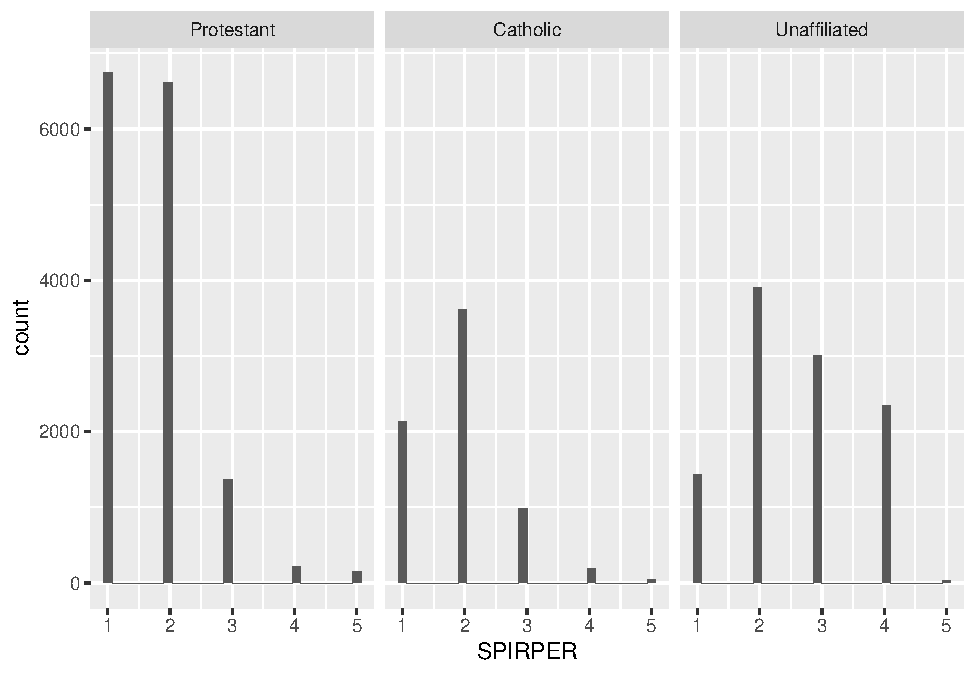
\includegraphics[keepaspectratio]{religion_project_files/figure-latex/unnamed-chunk-3-1.pdf}}
\pandocbounded{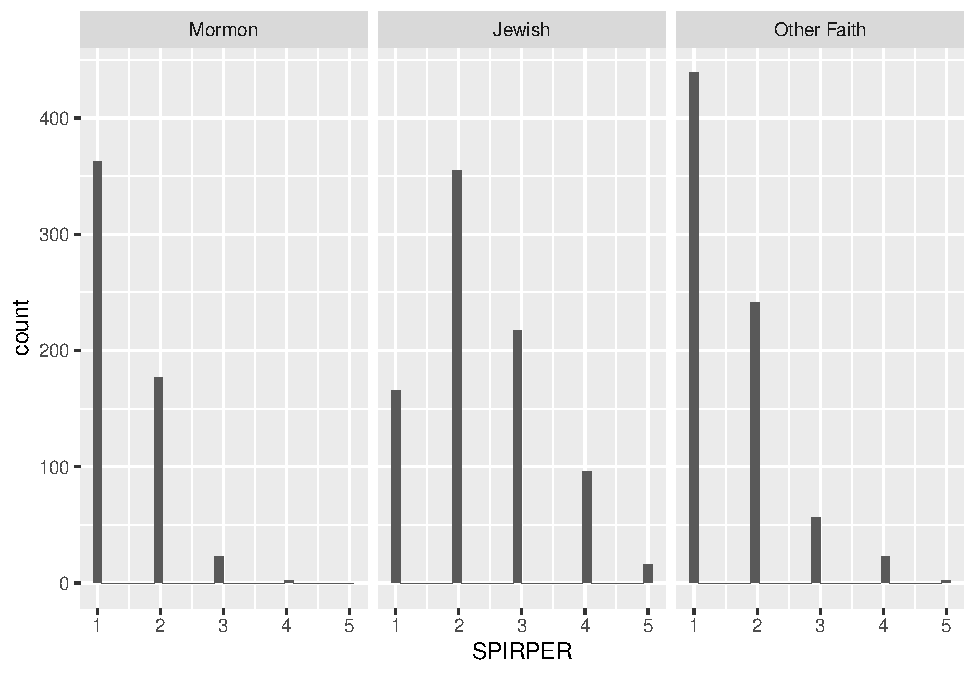
\includegraphics[keepaspectratio]{religion_project_files/figure-latex/unnamed-chunk-3-2.pdf}}
\pandocbounded{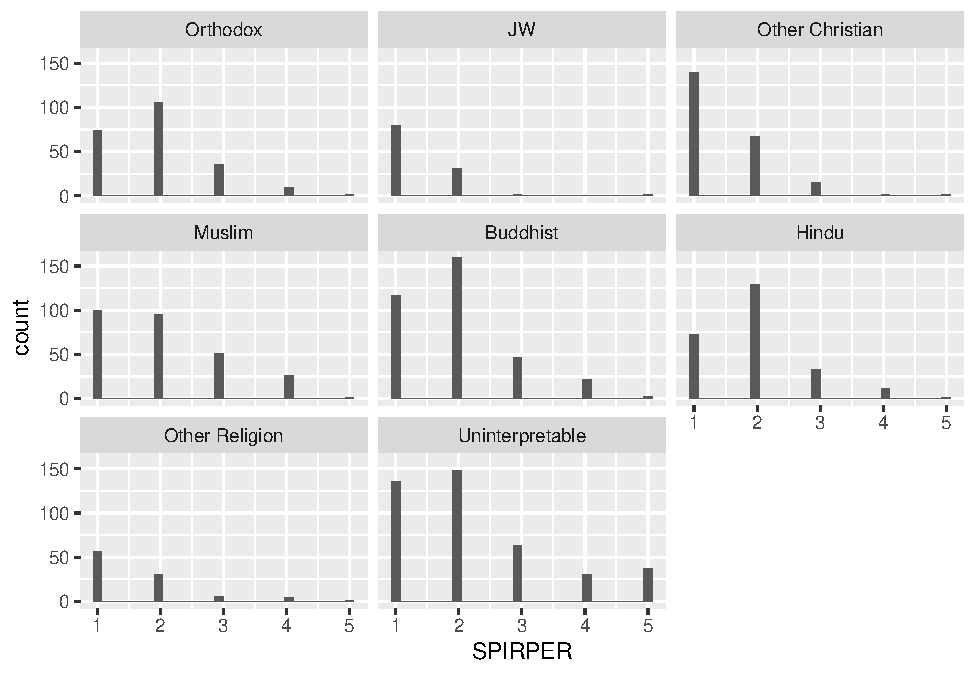
\includegraphics[keepaspectratio]{religion_project_files/figure-latex/unnamed-chunk-3-3.pdf}}

The spread for religiosity is shifted more to the higher (less
religious) values than spirituality: there were only two religions where
the plurality (largest spike) was 1 (most religious).

\pandocbounded{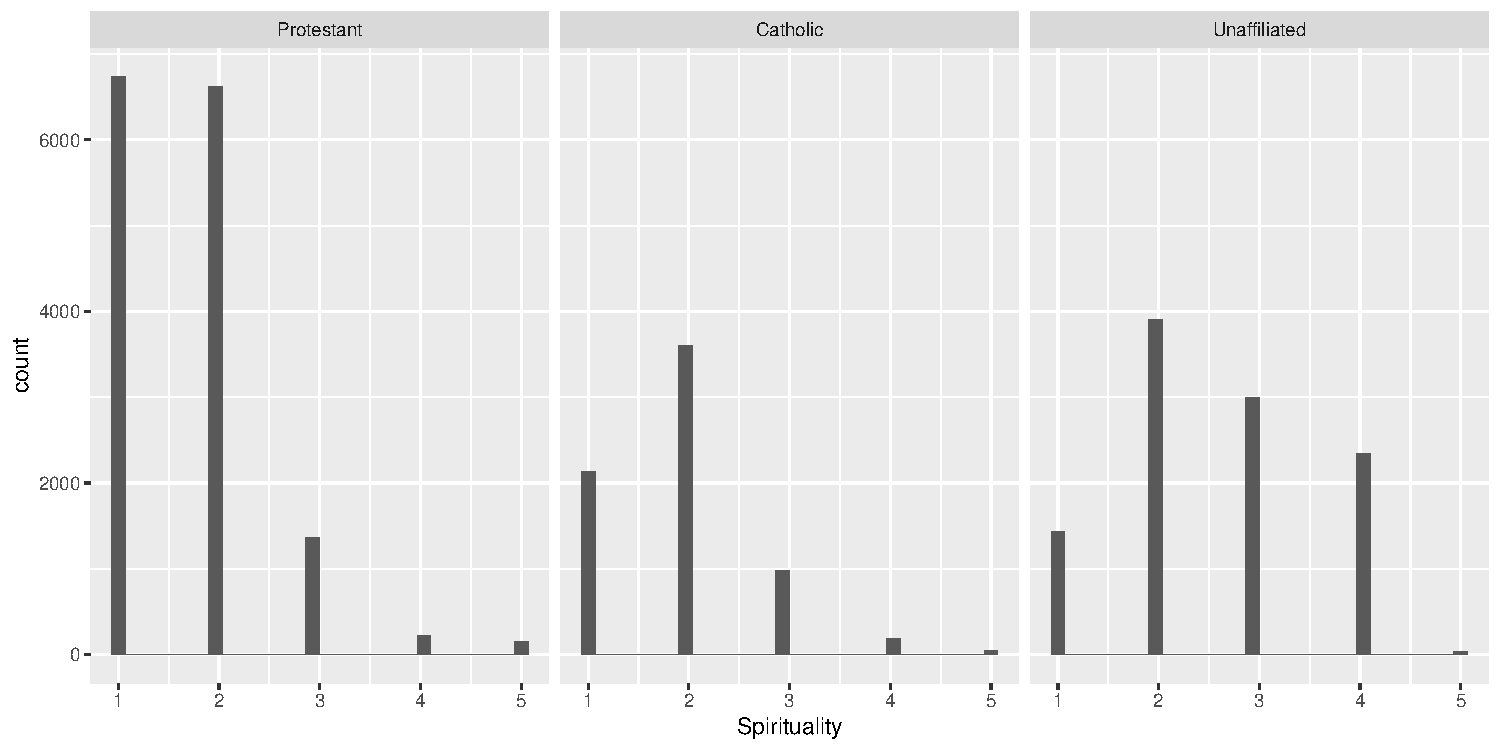
\includegraphics[keepaspectratio]{religion_project_files/figure-latex/unnamed-chunk-4-1.pdf}}
\pandocbounded{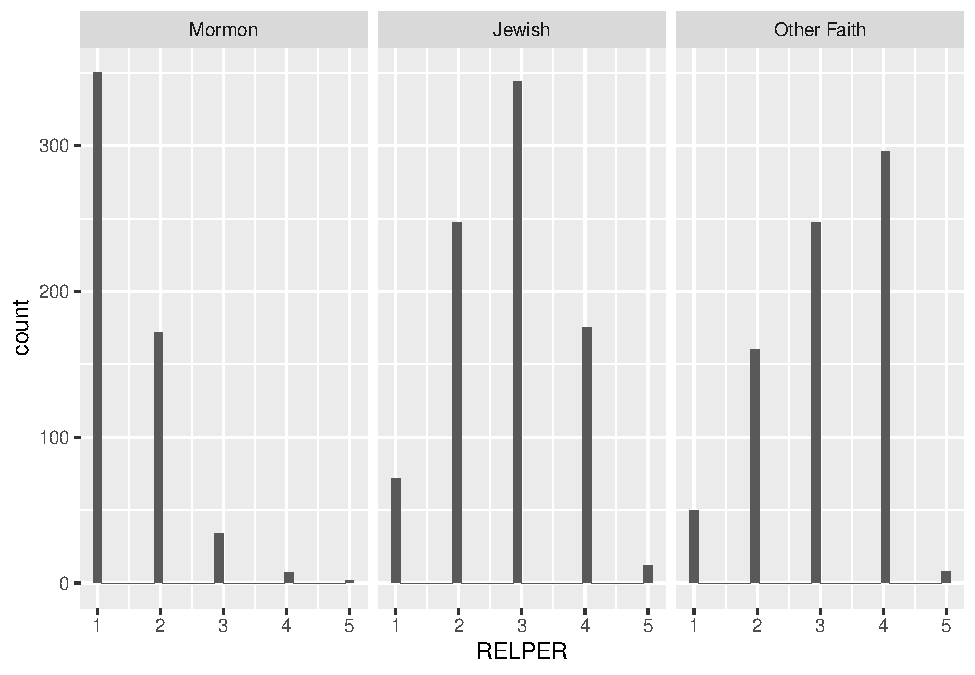
\includegraphics[keepaspectratio]{religion_project_files/figure-latex/unnamed-chunk-4-2.pdf}}
\pandocbounded{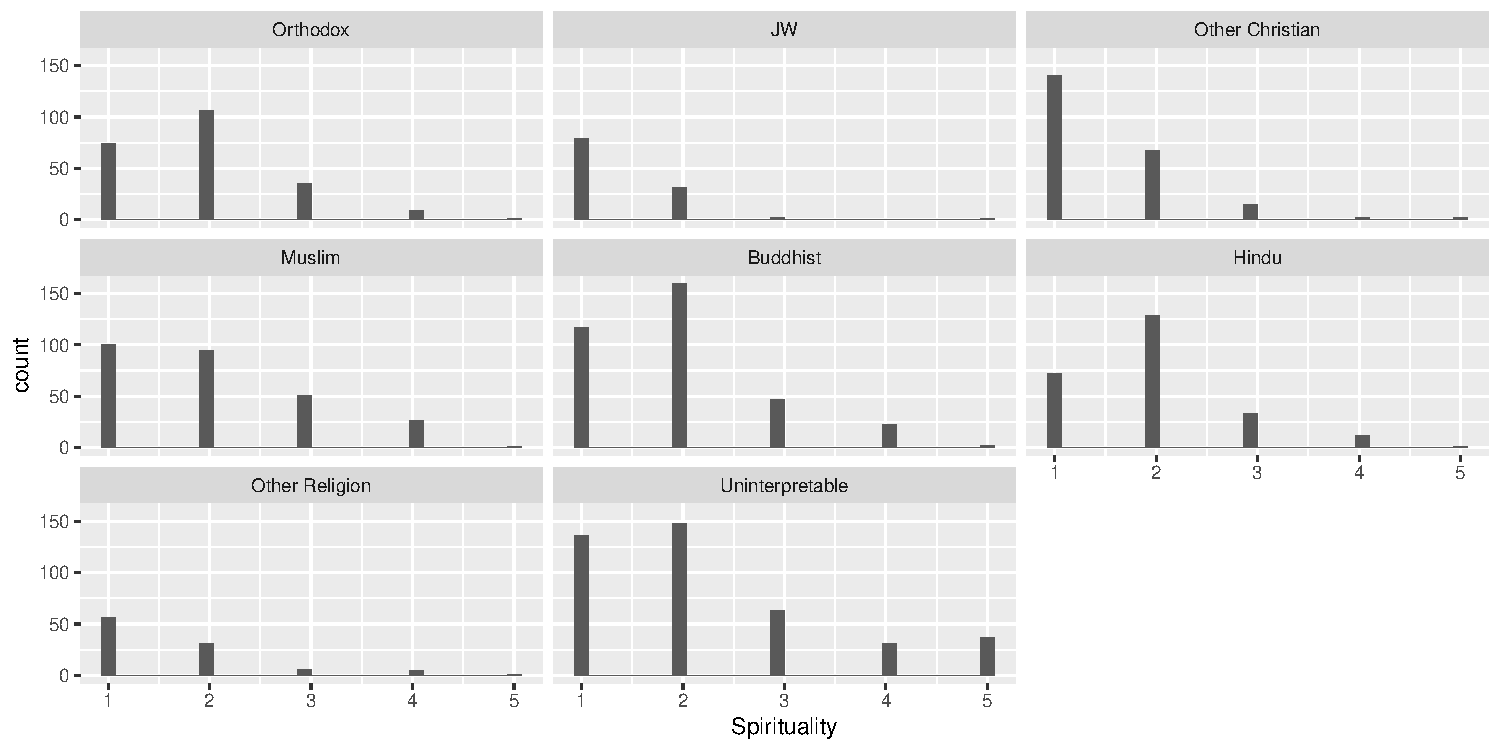
\includegraphics[keepaspectratio]{religion_project_files/figure-latex/unnamed-chunk-4-3.pdf}}

\section{Statistical Analysis}\label{statistical-analysis}

To formally investigate the relationships suggested by the exploratory
data analysis, we apply several statistical methods, including analysis
of variance (ANOVA), correlation analysis, simple linear regression, and
multiple linear regression. These methods allow us to test for group
differences, measure associations between variables, and identify key
predictors of religiosity.

\subsection{Section 1: Group
Differences}\label{section-1-group-differences}

We begin by examining whether religiosity differs across religious
traditions.

Hypothesis Test: \(H_0\): All religious groups have the same mean
religiosity.

\(H_a\): At least one group's mean is different.

\begin{verbatim}
##                Df Sum Sq Mean Sq F value Pr(>F)    
## CURREL         13  17394  1338.0    2247 <2e-16 ***
## Residuals   36590  21785     0.6                   
## ---
## Signif. codes:  0 '***' 0.001 '**' 0.01 '*' 0.05 '.' 0.1 ' ' 1
\end{verbatim}

\begin{verbatim}
## # A tibble: 14 x 4
##    CURREL          mean_religiosity sd_religiosity     n
##    <fct>                      <dbl>          <dbl> <int>
##  1 JW                          1.38          0.631   113
##  2 Mormon                      1.46          0.667   563
##  3 Protestant                  1.94          0.786 14949
##  4 Muslim                      2.01          0.882   272
##  5 Catholic                    2.06          0.743  6928
##  6 Orthodox                    2.12          0.776   223
##  7 Hindu                       2.21          0.752   246
##  8 Other Christian             2.39          0.959   224
##  9 Other Religion              2.65          1.03     99
## 10 Buddhist                    2.65          0.891   344
## 11 Uninterpretable             2.72          0.980   368
## 12 Jewish                      2.74          0.884   838
## 13 Other Faith                 3.05          0.933   753
## 14 Unaffiliated                3.48          0.731 10684
\end{verbatim}

The ANOVA results indicate that we reject the null hypothesis, as the
p-value is less than 0.05. This suggests that religiosity differs
significantly across religious traditions.

To further examine these differences, we computed the mean religiosity
score for each group. Religiosity is measured on a scale from 1 (very
religious) to 4 (not at all religious), excluding responses coded as 5
(don't know/refused). Because lower values indicate higher religiosity,
groups with lower mean scores are more religious on average. The results
show that Protestants have lower mean religiosity scores than Catholics
and the unaffiliated, indicating higher average religiosity, while the
unaffiliated group reports the highest mean scores, indicating the
lowest levels of religiosity.

Protestants, Catholics, and the unaffiliated also have the largest
sample sizes, making these estimates more reliable. The standard
deviations, which range approximately from 0.5 to 1, suggest a moderate
level of variation in religiosity within each group.

\pandocbounded{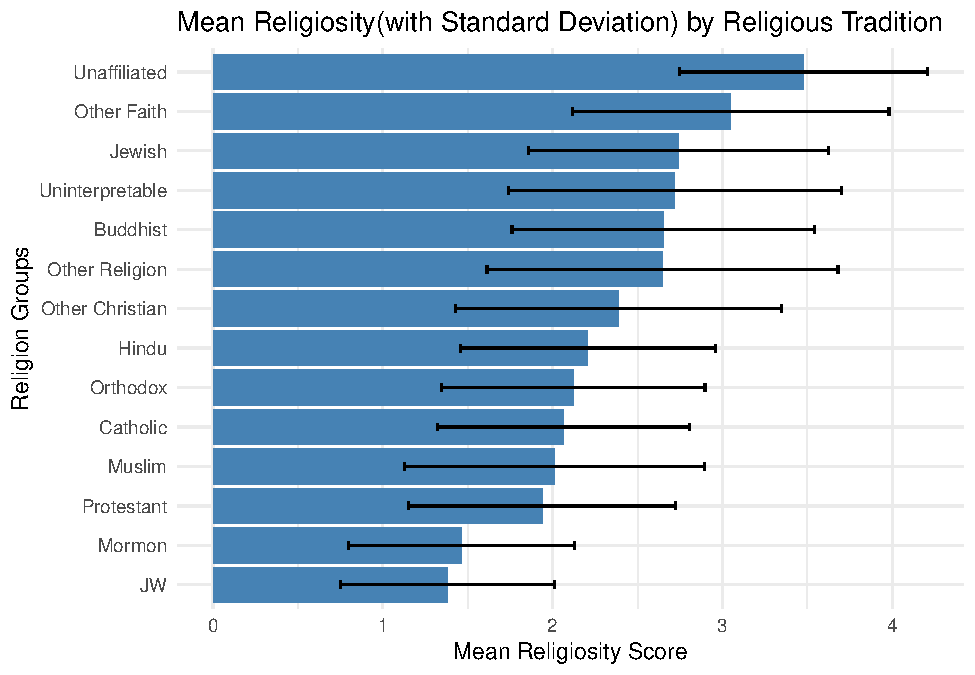
\includegraphics[keepaspectratio]{religion_project_files/figure-latex/unnamed-chunk-6-1.pdf}}

Check Assumptions for ANOVA: 1. Independence

\begin{enumerate}
\def\labelenumi{\arabic{enumi}.}
\setcounter{enumi}{1}
\item
  Normality within groups
\item
  Common variance
\end{enumerate}

\pandocbounded{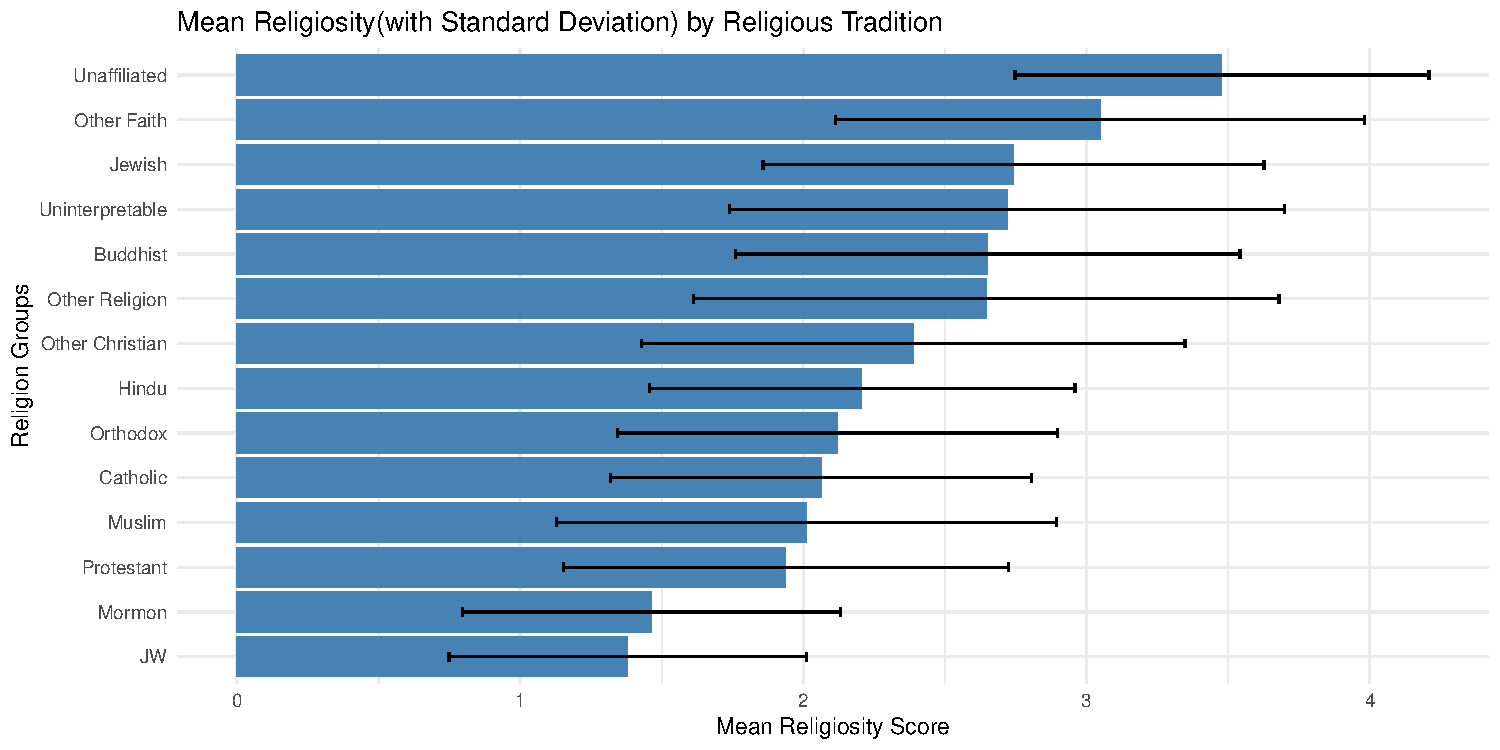
\includegraphics[keepaspectratio]{religion_project_files/figure-latex/unnamed-chunk-7-1.pdf}}

Independence is assumed based on the sampling design of the dataset.

A boxplot of religiosity scores was used to examine the distribution and
variability of religiosity across religious traditions. The plot shows
the median, interquartile range, and potential outliers for each group.

The distributions appear reasonably symmetric within most groups, with
no extreme deviations, suggesting that the assumption of approximate
normality is reasonable. In addition, the spread of scores across groups
is relatively similar, providing preliminary evidence that the
assumption of equal variances is satisfied.

\subsection{Section 2: Spirituality vs
Religiosity}\label{section-2-spirituality-vs-religiosity}

Next, we examine the relationship between spirituality and religiosity,
as the exploratory data analysis suggested that even unaffiliated
individuals report relatively high levels of spirituality.

\begin{verbatim}
## [1] 0.561914
\end{verbatim}

\begin{verbatim}
## 
## Call:
## lm(formula = RELPER ~ SPIRPER, data = data_no5)
## 
## Residuals:
##     Min      1Q  Median      3Q     Max 
## -2.7564 -0.4704 -0.1134  0.5296  2.1726 
## 
## Coefficients:
##             Estimate Std. Error t value Pr(>|t|)    
## (Intercept) 1.184407   0.010869   109.0   <2e-16 ***
## SPIRPER     0.642997   0.004959   129.7   <2e-16 ***
## ---
## Signif. codes:  0 '***' 0.001 '**' 0.01 '*' 0.05 '.' 0.1 ' ' 1
## 
## Residual standard error: 0.8557 on 36437 degrees of freedom
## Multiple R-squared:  0.3157, Adjusted R-squared:  0.3157 
## F-statistic: 1.681e+04 on 1 and 36437 DF,  p-value: < 2.2e-16
\end{verbatim}

A correlation analysis was conducted between religiosity (RELPER) and
spirituality (SPIRPER), excluding missing responses. The result is
0.562, indicating a moderate positive relationship between the two
variables. This suggests that higher levels of spirituality are
associated with higher religiosity scores. Given that higher religiosity
scores correspond to lower levels of religiosity (1 = very religious, 4
= not at all religious), this indicates that higher spirituality is
associated with lower reported religiosity.

A simple linear regression further examined this relationship. The
results show that spirituality is a statistically significant predictor
of religiosity (p \textless{} 0.05). The coefficient indicates that a
one-unit increase in spirituality is associated with an increase in
religiosity score. The model explains approximately 31.57\% (\(R^2\) =
0.3157) of the variation in religiosity, suggesting a moderate
relationship.

\pandocbounded{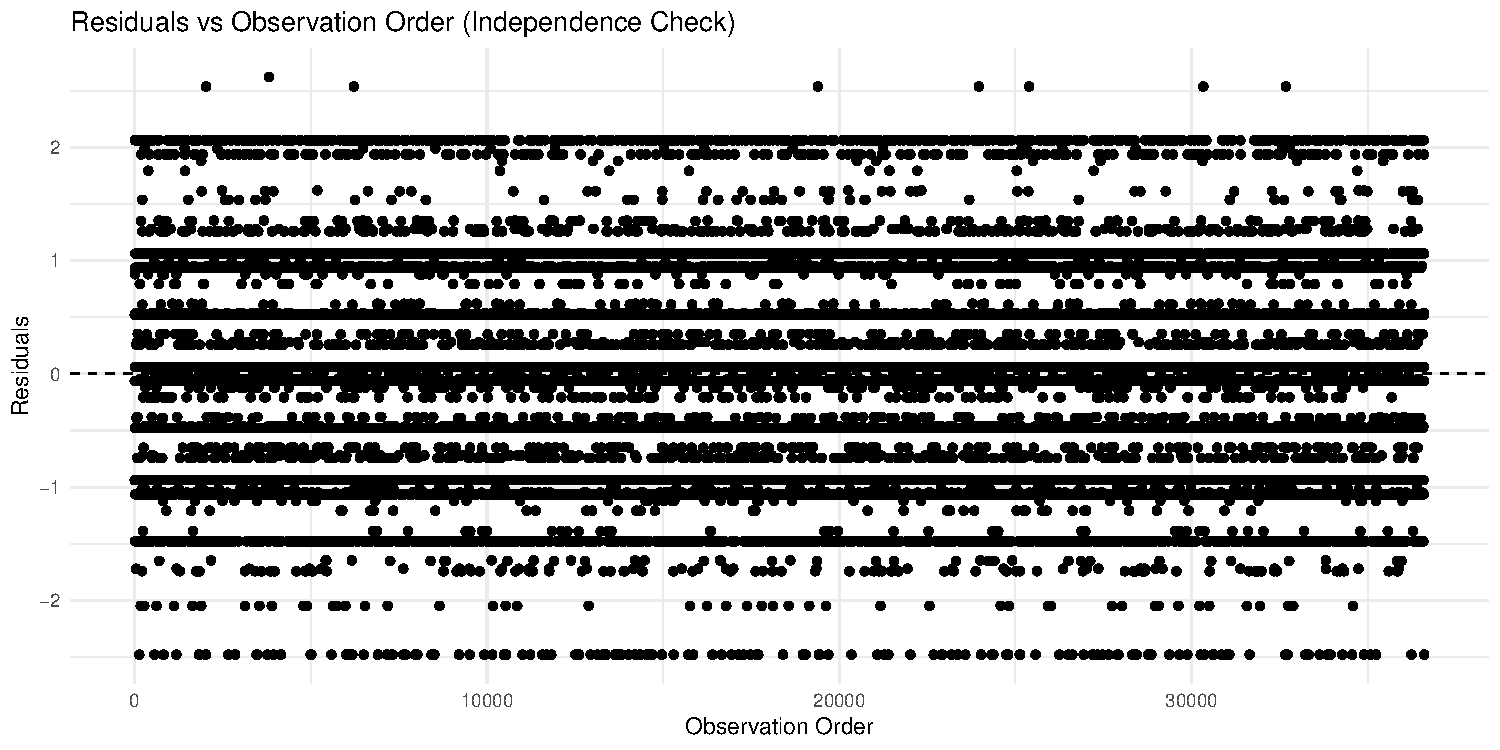
\includegraphics[keepaspectratio]{religion_project_files/figure-latex/unnamed-chunk-9-1.pdf}}

As spirituality increases, religiosity score increased, indicating lower
religiosity. A jittered scatterplot with a fitted linear regression line
was used to visualize the relationship between spirituality and
religiosity. Jittering was applied to help with data visualization due
to the discrete nature of the 1--4 response scale.

\subsection{Section 3: Behavioral
Predictors}\label{section-3-behavioral-predictors}

While spirituality captures internal beliefs, religiosity may also be
influenced by observable behaviors such as attendance and prayer. We
therefore examine whether these behavioral variables are significant
predictors of religiosity.

Data description:

ATTNDPERRLS measures frequency of attendance at religious services (1 =
more than once a week, 6 = never).

PRAY measures frequency of prayer outside services (1 = several times a
day, 7 = never).

PRAC\_B measures frequency of reading scripture (1 = at least once a
week, 5 = never).

PRAC\_D measures frequency of sharing religious views with people of
other faiths (1 = at least once a week, 5 = never).

We test whether behavioral factors (attendance, prayer frequency, and
religious practices) significantly predict religiosity.

Hypothesis Test: \(H_0\): That none of these behaviors are associated
with religiosity \(H_a\): That at least one behavioral variable
significantly predicts religiosity.

The results from the full model indicate that attendance (ATTNDPERRLS),
prayer frequency (PRAY), and scripture reading (PRAC\_B) are
statistically significant predictors of religiosity (p \textless{}
0.05). Given the coding of religiosity (higher values indicate lower
religiosity), these results suggest that more frequent religious
practices are associated with higher levels of religiosity (i.e., more
religious behavior). In contrast, PRAC\_D is not statistically
significant, suggesting that sharing religious views with others does
not have a measurable relationship with religiosity in this model.

The model explains approximately 58.56\% (\(R^2\) = 0.5856) of the
variation in religiosity, indicating a relatively strong relationship
between behavioral practices and religiosity.

The results from the Protestant model indicate that attendance
(ATTNDPERRLS), prayer frequency (PRAY), scripture reading (PRAC\_B), and
sharing religious views (PRAC\_D) are statistically significant
predictors of religiosity (p \textless{} 0.05). Given the coding of
religiosity, where higher values indicate lower levels of religiosity,
these results suggest that more frequent religious practices are
associated with lower religiosity scores, indicating higher levels of
religious engagement.

The model explains approximately 27.34\% (\(R^2\) = 0.2734) of the
variation in religiosity, suggesting a moderate relationship between
behavioral practices and religiosity within the Protestant subsample.

The results from the Catholic model indicate that attendance
(ATTNDPERRLS), prayer frequency (PRAY), scripture reading (PRAC\_B), and
sharing religious views (PRAC\_D) are statistically significant
predictors of religiosity (p \textless{} 0.05). Given the coding of
religiosity, where higher values indicate lower levels of religiosity,
these results suggest that more frequent religious practices are
associated with lower religiosity scores, indicating higher levels of
religious engagement.

The model explains approximately 47.64\% (\(R^2\) = 0.4764) of the
variation in religiosity, suggesting a relatively strong relationship
between behavioral practices and religiosity within the Catholic
subsample.

The results from the Muslim model indicate that attendance
(ATTNDPERRLS), prayer frequency (PRAY), and scripture reading (PRAC\_B)
are statistically significant predictors of religiosity (p \textless{}
0.05). Given the coding of religiosity, where higher values indicate
lower levels of religiosity, these results suggest that more frequent
religious practices are associated with lower religiosity scores,
indicating higher levels of religious engagement. In contrast, PRAC\_D
is not statistically significant, suggesting that sharing religious
views with others does not have a measurable relationship with
religiosity in this model.

The model explains approximately 40.63\% (\(R^2\) = 0.4063) of the
variation in religiosity, suggesting a moderate to relatively strong
relationship between behavioral practices and religiosity within the
Muslim subsample.

The results from the Unaffiliated model indicate that some behavioral
variables are statistically significant predictors of religiosity (p
\textless{} 0.05). Given the coding of religiosity, where higher values
indicate lower levels of religiosity, these results suggest that more
frequent religious practices are associated with lower religiosity
scores, indicating higher levels of religious engagement.

The model explains approximately 38.84\% (\(R^2\) = 0.3884) of the
variation in religiosity, suggesting a moderate relationship between
behavioral practices and religiosity within the Unaffiliated subsample.

\subsection{Section 4: Political Predictors of
Religiosity}\label{section-4-political-predictors-of-religiosity}

It would appear that removal of the 99s which represent those who did
not answer made a substantial difference on the fit of the model.
Furthermore, support for gay marriage predicts religiosity well, as does
support for transgender individuals. However, acceptance of
homosexuality is an incredibly poor predictor of religiosity in the body
public.

Alternatively, support for abortion, homosexuality, and gay marriage
predicts spirituality but support for transgender individuals does not
predict spirituality.

While support for abortion, same sex marriage, and homosexuality is a
statistically significant predictor of religiosity in Catholics and
people who are unaffiliated, support for these causes is not
statistically significant in predicting religiosity in Protestants.
Interestingly, greater acceptance of transgender individuals cannot be
used to predict religiosity in people who are unaffiliated.

\subsection{Section 5: Comprehensive
Model}\label{section-5-comprehensive-model}

Finally, we construct a comprehensive model using 27 variables that
incorporates behavioral measures, belief variables, and religious
affiliation to determine which factors are most important in predicting
religiosity.

With an \(R^2\) of 0.71, we have pretty good confidence that this model
can predict religiosity in individuals. An \(R^2\) of 0.71 tells us that
71\% of variance can be explained by the model and the variables that we
presented it with. The results for spirituality were quite a bit lower,
however, with an \(R^2\) of just 43\%.

Check for Assumptions of Regression: 1. Linearity 2. Nearly normal
residuals 3. Constant variability

Looking at the p-values for the religiosity model, there were quite a
few variables that were not impactful in predicting religiosity. These
included FRMREL, RELTRAD, CURREL, CHATTEND, MARITAL, BIRTHDECADE, HISP,
RACECMB, E2, USGEN, REG, PARTY, and GENDER. When these variables were
removed, the \(R^2\) value decreased to .64.

\section{Conclusions}\label{conclusions}

Across both the full sample and some religious subsamples, behavioral
factors---including attendance, prayer frequency, and scripture
reading---consistently emerge as significant predictors of religiosity.
These findings suggest that religiosity is strongly shaped by observable
religious practices, rather than being solely an internal belief system.

However, the strength of these relationships varies across religious
traditions. The Catholic and Muslim subsamples show relatively stronger
explanatory power, while the Protestant model shows a weaker
relationship between behaviors and religiosity. The Unaffiliated group
also demonstrates that behavioral practices remain relevant even in the
absence of formal religious affiliation.

Overall, the results indicate that religiosity is best understood as a
behaviorally structured phenomenon, but the degree to which behavior
predicts religiosity differs across religious traditions. This suggests
that religious tradition plays a moderating role in shaping how
behaviors translate into levels of religiosity.

Similarly, depending on the religious tradition, certain political
beliefs seemed to show a moderate correlation with religiosity and
spirituality.

For the full models, religiosity was much easier to predict based on the
behavioral, political and religious beliefs and factors than
spirituality. One reason that this may be the case is potentially due to
religious affiliation (with higher religiosity being already more rare)
being associated with a specific set of beliefs that one subscribes to.
On the other hand, one can claim to be spiritual to a certain extent,
but this term is more vague in what it describes. Many classify
themselves as ``spiritual but not religious,'' a category that denotes
vague spiritual feelings without adherence to a specific religion. It is
important to note that the analogous ``religious but not spiritual''
designation is almost far less common than its counterpart and mostly
nonsensical.

\end{document}
